% IN51 - Particle System project report
% Spring 2014
% Authors : Adrien Berthet, Gautier Claisse and Karim Naaji

%----------------------------------------------------------------------------------------
%	PACKAGES AND DOCUMENT CONFIGURATIONS
%----------------------------------------------------------------------------------------

\documentclass[a4paper,10pt]{report}
\usepackage[margin=1.3in]{geometry}
\usepackage[utf8x]{inputenc}
\usepackage[T1]{fontenc}
\usepackage[french]{babel}
\usepackage{color,colortbl}
\usepackage{phdthesis}	% Much beautiful
\usepackage{fancyhdr}
\usepackage{graphicx}
\usepackage{hyphenat}	% Caesura

% Code Coloring with minted, use it as follow :
% \begin{figure}
%	\begin{minted}[bgcolor=bg,tabsize=4]{c}
%		printf("hello");
%	\end{minted}
% \end{figure}
\usepackage{minted}
\definecolor{bg}{rgb}{0.95,0.95,0.95}

\renewcommand*\rmdefault{phv} % Helvetica yeah yeah yeah

\setlength\parindent{0pt} % Removes all indentation from paragraphs

%----------------------------------------------------------------------------------------
%	DOCUMENT INFORMATION
%----------------------------------------------------------------------------------------

\title{Système de particules\\Projet d'IN55}
\author{Adrien \bsc{Berthet}, Gautier \bsc{Claisse} et Karim \bsc{Naaji}}
\date{\bsc{Printemps} 2014}

\begin{document}

\maketitle

%----------------------------------------------------------------------------------------
%	CONTENT
%----------------------------------------------------------------------------------------

% INTRODUCTION
\chapter*{Introduction}


% PROJECT PRESENTATION
\chapter{Présentation du projet}

\section{Objectifs fixés}

Le sujet choisi avait pour consignes de paramétrer le rendu de particules
constitutives d'un phénomène physique (fumée, feu, eau) et de simuler leur
rendu dans une scène. La gestion de la physique doit être réalisée avec des
calculs GPU, c'est à dire avec GLSL et des shaders.\\

À partir de ces consignes, nous avons décidé de réaliser un programme de rendu
contenant un émetteur de particules. Cet objet sert de point d'émission aux
particules, qui vont alors se déplacer suivant différents \emph{patterns} précis
: par exemple un cône, une pyramide ou encore une sphère (émission non limitée 
dans tous les sens). Pour ne pas avoir d'attente trop haute, ces objectifs sont
les principaux fixés. D'autres, considérés comme secondaires, ont été évoqués.
Il serait ensuite possible de placer plusieurs émetteurs (directement par le 
code ou par l'utilisateur via la souris) et ainsi cela permettrait d'observer la
réaction de particules se rencontrant entre elles.\\

\section{Résultat final}

Le rendu final est celui escompté : deux types d'émissions sont disponibles
(émissions sphérique et cônique) et également un « plan » de particules qui a un
mouvement semblable à des vagues. L'ensemble des tranformations des particules a
été réalisée à travers un ensemble de /emph{shaders}, que cela soit pour les
mouvements comme pour les couleurs. L'interface est également présente, même si
limitée, par manque de temps principalement et peu de connaissance sur le sujet
des widgets Qt (voir paragraphe \ref{gui}).

% We need screen cap here pls
\begin{figure}[h]
	\begin{center}
		%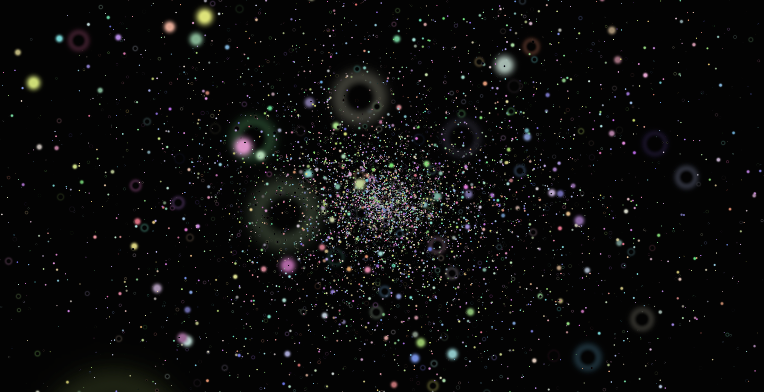
\includegraphics[width=0.2\textwidth]{img/21-sphere.png}
	\end{center}
	\caption{Rendu à émission spérique}
\end{figure}

\begin{figure}[h]
	\begin{center}
		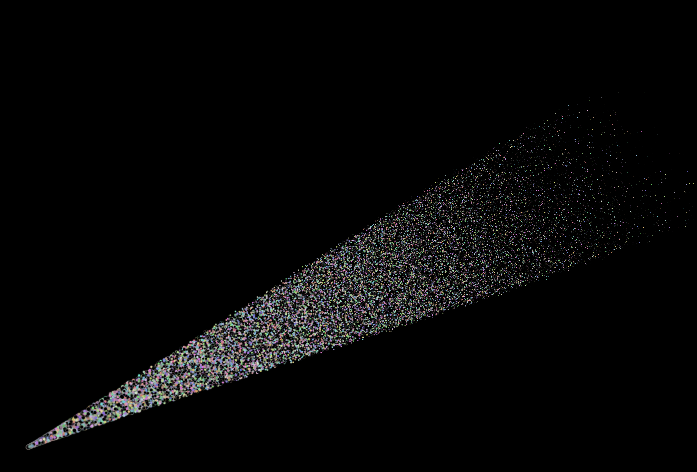
\includegraphics[width=0.8\textwidth]{img/22-cone.png}
	\end{center}
	\caption{Rendu avec diffusion cônique}
\end{figure}

\begin{figure}[h]
	\begin{center}
		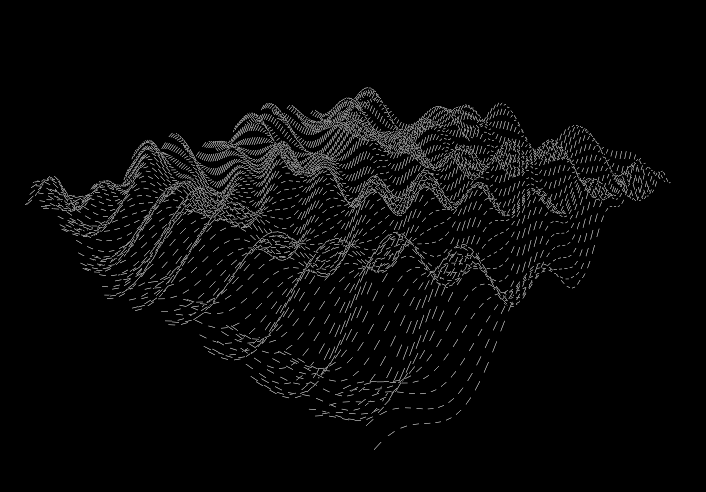
\includegraphics[width=0.8\textwidth]{img/23-waves.png}
	\end{center}
	\caption{Rendu avec des vagues}
\end{figure}


% MODELISATION / IMPLEMENTATION
\chapter{Modélisation et implémentation}

\section{Fonctionnement global}

Résumé simplement, on peut dire qu'il y a création d'une scène dans
laquelle on met des noeuds. Ces noeuds correspondent à des objets qui seront contenus
dans la scène. Comme dit précédemment, nous avons deux types finaux pour les noeuds:
l'\emph{EmitterNode} et le \emph{WaveParticleNode}. \\

Les deux ont un comportement identique. Ils vont créer des vertex et leur donner des
attributs initiaux. Ces attributs peuvent être une position, une vitesse, une couleur
ou encore un temps de vie par exemple. Lorsque les vertex sont initialisés, le noeud ne
va plus réellement s'occuper d'eux. En effet, ils sont ensuite gérés uniquement par des
shaders. Tous les traitements ultérieurs subis par les vertex sont effectués par des 
shaders. Les actions à exercer sur ces vertex sont calculées à partir des attributs initiaux
de chaque vertex et du temps. L'exemple le plus visuel est la position. Ainsi,
il n'est par exemple pas possible de gérer les collisions entre particules mais c'est le GPU qui gère
tous ces calculs.\\

L'initialisation de ces attributs est simplifiée par l'introduction de \emph{Samplers}.
Ces \emph{Samplers} servent uniquement à générer des données de manière aléatoire. Par exemple
le \emph{ConeSampler} va simplement générer des vecteurs de directions (partant de la base du cône
en prenant en compte son ouverture).

\begin{figure}[h]
	\begin{center}
		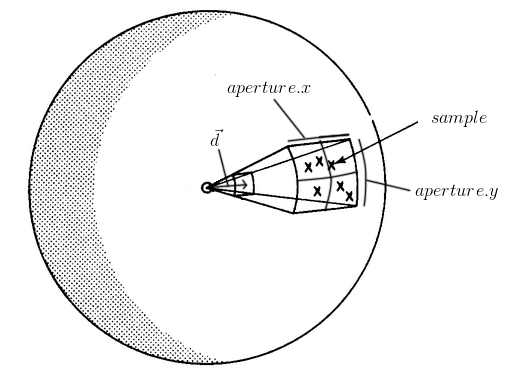
\includegraphics[width=0.5\textwidth]{img/conesampler.png}
	\end{center}
	\caption{Shéma du \emph{ConeSampler}}
\end{figure}

L'introduction du \emph{ShaderManager} a été très utile. C'est l'objet qui va gérer tous les
shaders utilisés dans le projet.

\begin{figure}[h]
	\begin{center}
		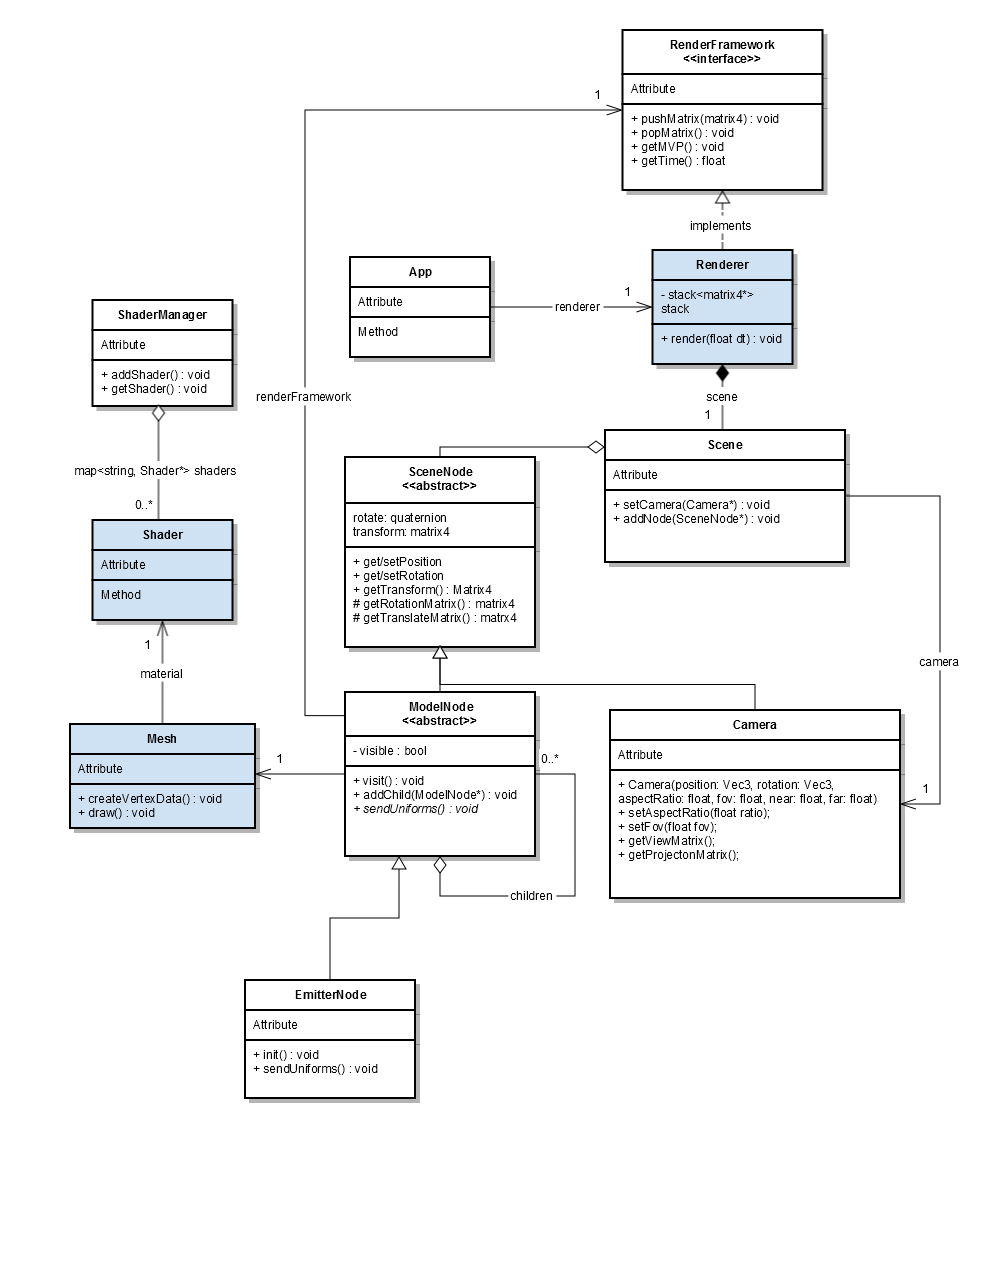
\includegraphics[width=\textwidth]{img/UML.png}
	\end{center}
	\caption{Diagramme UML du projet}
\end{figure}

% Continuer sur des spécifités spécifiques


% PROBLEMS / DIFFICULTIES
\chapter{Difficultés rencontrées}

% TODO Zarov

% Gestion de l'alpha, Positionnement de la Camera, Rotation de la camera avec la
% souris, GUI


% POSSIBLE IMPROVEMENTS
\chapter{Améliorations possibles}

% TODO Lunpe
% Ajout de trajectoires différentes, gestion de plusieurs points d'émission,
% intégration à un environnement, flexibilité

Bien qu'on puisse considérer le projet comme fini, il y a toujours des choses
que nous pourrions ajouter ou améliorer. Ce sont des améliorations qui sont
dans le domaine du nice-to-have et que nous n'avons pas implémenté.

\section{Ajout de trajectoires différentes}
Nous avons une base de shaders très simples qui permettent de déplacer nos
particules correctement. Cela dit, ces déplacements ne sont pas toujours très
impressionnants. Une amélioration possible serait d'ajouter plein de types de
forces différentes et de sélectionner lesquelles appliquer à nos particules
(gravité, force radiale, rappel vers le point d'émission, ajout d'un spin à la
trajectoire ou autres). Certaines de ces choses seraient faciles à implémenter (gravité
ou rappel vers le point d'émission) alors que d'autres demanderaient plus de réflexion
afin de déterminer les bonne forces (et dans quelles directions) appliquer uniquement
en fonction du temps. Il serait ainsi possible de conjuguer toutes ces forces
afin d'avoir des comportements plus poussés.

\section{Gestion de plusieurs points d'émission}
Actuellement, la scène ne comporte qu'un noeud de particules. Augmenter ce
nombre pourrait être intéressant autant d'un point de vue visuel qu'utilitaire.
En effet, monter un système de particules possédant plusieurs sources ou types
de particules permet de faire des choses bien plus aguichantes qu'un simple émetteur
de particules. La raison pour laquelle nous n'avons pas implémenté cette fonction est
que, derrière ses airs triviaux, elle nous pose un problème dans la gestion des shaders.
En effet, créer un noeud deux fois recquiert d'utiliser le shader deux fois, et en faisant
cela on crée le même shader plusieurs fois ce qui n'est pas possible dans notre cas.

\section{Intégration à un environnement}
La dernière amélioration notoire que nous avons pensé faire est d'intégrer nos systèmes
de particules dans un environnement comportant d'autre objets 3D. On pourrait donner
en exemple le fait d'avoir un modèle de torche et de placer un émetteur de particules
ayant des textures se rapprochant de la fumée afin d'avoir l'impression que la torche fume.
Cependant, il serait aussi possible de faire une intégration à un environnement bien plus poussée.
En effet, en passant des objets 3D simples au vertex shader, il serait possible de faire
intéragir nos particules et ces objets: des balles qui rebondissent au sol par exemple. 


% CONCLUSION
\chapter*{Conclusion}


\end{document}